%%%%%%%%%%%%%%%%%%%%%%%%%%%%%%%%%%%%%%%%%
% baposter Landscape Poster
% LaTeX Template
% Version 1.0 (11/06/13)
%
% baposter Class Created by:
% Brian Amberg (baposter@brian-amberg.de)
%
% This template has been downloaded from:
% http://www.LaTeXTemplates.com
%
% License:
% CC BY-NC-SA 3.0 (http://creativecommons.org/licenses/by-nc-sa/3.0/)
%
%%%%%%%%%%%%%%%%%%%%%%%%%%%%%%%%%%%%%%%%%

%----------------------------------------------------------------------------------------
%	PACKAGES AND OTHER DOCUMENT CONFIGURATIONS
%----------------------------------------------------------------------------------------

\documentclass[landscape,a0paper,fontscale=0.3]{baposter} % Adjust the font scale/size here

\usepackage{graphicx} % Required for including images
\graphicspath{{/home/alli/projects/talks/figures/}} % Directory in which figures are stored

\usepackage{amsmath} % For typesetting math
\usepackage{amssymb} % Adds new symbols to be used in math mode
\usepackage{booktabs} % Top and bottom rules for tables
\usepackage{enumitem} % Used to reduce itemize/enumerate spacing
\usepackage{palatino} % Use the Palatino font
\usepackage[font=small,labelfont=bf]{caption} % Required for specifying captions to tables and figures

\usepackage{multicol} % Required for multiple columns
\usepackage{subcaption}
\setlength{\columnsep}{1.5em} % Slightly increase the space between columns
\setlength{\columnseprule}{0mm} % No horizontal rule between columns


\usepackage{tikz} % Required for flow chart
\usetikzlibrary{shapes,arrows} % Tikz libraries required for the flow chart in the template

\newcommand{\compresslist}{ % Define a command to reduce spacing within itemize/enumerate environments, this is used right after \begin{itemize} or \begin{enumerate}
\setlength{\itemsep}{1pt}
\setlength{\parskip}{0pt}
\setlength{\parsep}{0pt}
}

\definecolor{lightblue}{rgb}{0.145,0.6666,1} % Defines the color used for content box headers
\definecolor{darkpurple}{rgb}{0.28,0.24,0.55}


\begin{document}

\begin{poster}
{
%headerborder=closed, % Adds a border around the header of content boxes
colspacing=1em, % Column spacing
columns=3,
bgColorOne=white, % Background color for the gradient on the left side of the poster
bgColorTwo=white, % Background color for the gradient on the right side of the poster
borderColor=lightblue, % Border color
headerColorOne=darkgray, % Background color for the header in the content boxes (left side)
headerColorTwo=darkpurple, % Background color for the header in the content boxes (right side)
headerFontColor=white, % Text color for the header text in the content boxes
boxColorOne=white, % Background color of the content boxes
%textborder=roundedleft, % Format of the border around content boxes, can be: none, bars, coils, triangles, rectangle, rounded, roundedsmall, roundedright or faded
textborder=none, % Format of the border around content boxes, can be: none, bars, coils, triangles, rectangle, rounded, roundedsmall, roundedright or faded
eyecatcher=true, % Set to false for ignoring the left logo in the title and move the title left
headerheight=0.1\textheight, % Height of the header
%headershape=roundedright, % Specify the rounded corner in the content box headers, can be: rectangle, small-rounded, roundedright, roundedleft or rounded
headershape=rounded, % Specify the rounded corner in the content box headers, can be: rectangle, small-rounded, roundedright, roundedleft or rounded
headerfont=\Large\bf\textsc, % Large, bold and sans serif font in the headers of content boxes
%textfont={\setlength{\parindent}{1.5em}}, % Uncomment for paragraph indentation
linewidth=2pt % Width of the border lines around content boxes
}
%----------------------------------------------------------------------------------------
%	TITLE SECTION 
%----------------------------------------------------------------------------------------
%
{\includegraphics[height=6em]{illinois_logo.jpg}} % First university/lab logo on the left
{{Controllable~~Billiards:~~Characterizing~~the~~Paths~~of~~Simple~~Mobile~~Robots}\vspace{-0.0em}} % Poster title
{Alexandra Q. Nilles, Israel Becerra, Steven M. LaValle  \hspace{15pt}\\ Department of Computer Science, University of Illinois, Urbana-Champaign} % Author names and institution
{
\includegraphics[height=8em]{/home/alli/projects/talks/figures/nsf1.jpg}} % Second university/lab logo on the right

%----------------------------------------------------------------------------------------
%	INTRODUCTION
%----------------------------------------------------------------------------------------

\headerbox{Motivation}{name=intro,column=0,row=0,span=1}{

\begin{itemize}
\item What kinds of tasks can very simple robots perform?

\item What are the minimal resources (sensing, actuation, computation time and
space) needed to complete tasks?

\item Can we make common robots (such as vacuums and warehouse) robots more efficient
and robust?
\end{itemize}


\begin{center}
\includegraphics[width=0.9\linewidth]{robot_brain.jpg}
\end{center}


}

%----------------------------------------------------------------------------------------
%	Question
%----------------------------------------------------------------------------------------

\headerbox{Robotic Tasks as Properties of Paths}{name=question,below=intro,column=0,span=1}{

\begin{itemize}\compresslist
\item {\bf Navigation:} From a set of starting states (which may be the entire
environment), the robot's path must end at the goal state(s).
\item {\bf Coverage:} The robot's path must meet some coverage criterion (ex: if
the robot has a lidar sensor with omnidirectional 5 meter radius, the robot will
scan the entire environment).
\item {\bf Patrolling:} The robot's path must be repeatable, and may also have
some coverage criterion.
\end{itemize}

}

%----------------------------------------------------------------------------------------
%	APPROACH
%----------------------------------------------------------------------------------------


\headerbox{Approach}{name=flow,column=0,span=1,below=question}{

Notice that many robots can travel forward in straight lines, identify when
they've reached a boundary (real or virtual), and turn in place!

Can we use billiards or similar models?

\begin{center}
\includegraphics[width=1\linewidth]{bounce_space_def.pdf}
\captionof{figure}{Outline of homology search and state mapping approach. Presence/absence patterns
that essential genes are less likely to be lost.}
\end{center}

}

%----------------------------------------------------------------------------------------
%	LIMIT CYCLES IN CONVEX POLYGONS
%----------------------------------------------------------------------------------------

\headerbox{Limit Cycles in Convex
Polygons}{name=convex,column=1,row=0,span=1}{

\begin{center}
\includegraphics[width=0.8\linewidth]{convex_fp.pdf}
\captionof{figure}{Consecutive-edge bouncing limit cycles exist and are computable for a range of $\theta$ in every convex polygon.}
\end{center}
}

%----------------------------------------------------------------------------------------
%	FORMAL METHODS
%----------------------------------------------------------------------------------------

\headerbox{The Role of Formal
Methods}{name=convex,column=1,span=1,below=convex}{

\begin{center}
\includegraphics[width=0.8\linewidth]{convex_fp.pdf}
\captionof{figure}{Consecutive-edge bouncing limit cycles exist and are computable for a range of $\theta$ in every convex polygon.}
\end{center}
}



%----------------------------------------------------------------------------------------
%	NONCONVEXITY
%----------------------------------------------------------------------------------------

\headerbox{Nonconvex Environments}{name=nonconvex,column=2,row=0,span=1}{ 

\begin{centering}
\includegraphics[width=0.9\linewidth]{nonconvex1.png}
\end{centering}

\begin{itemize}
\item Decompose nonconvex polygons by extending edges meeting in reflex angles
\item Limit cycles will exist 
\end{itemize}


}

%----------------------------------------------------------------------------------------
%	RESULTS 2
%----------------------------------------------------------------------------------------
%\headerbox{Results: Reconstruciton}{name=results_2,column=2,span=1,below=circos}{ 
\headerbox{Chaotic Dynamics: Coverage
Properties}{name=chaos,column=2,span=1,below=nonconvex}{ 


%%
%%\begin{multicols}{2}
\begin{center}
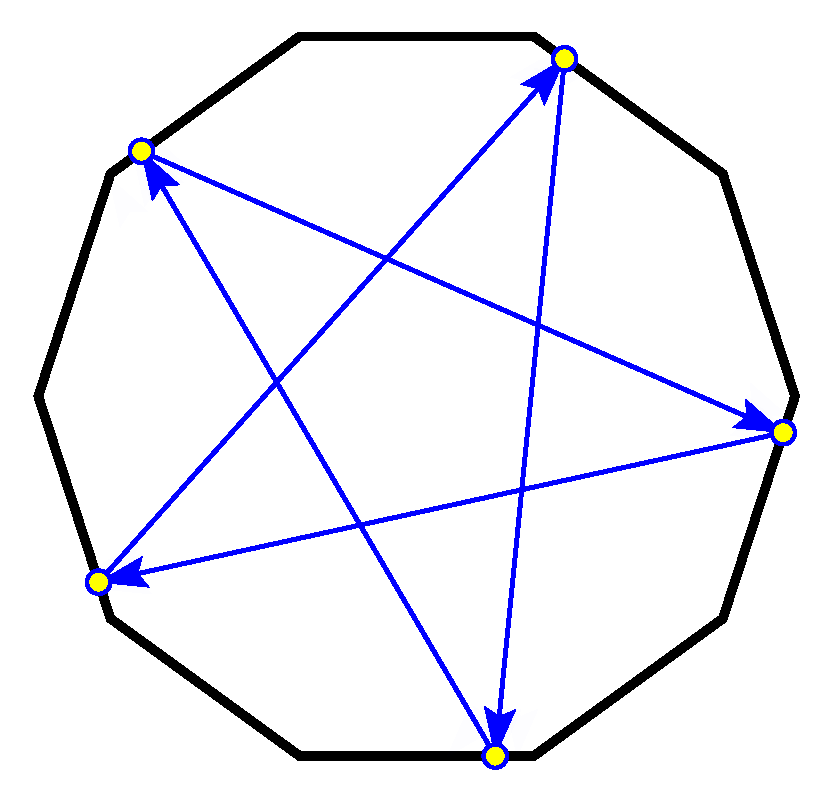
\includegraphics[width=0.5\linewidth]{../figs/nonagon_neg0pt8rad_skip3.pdf}
\captionof{figure}{Maximum parsimony tree made in PAUP\* (Swofford, et al 2017) from
presence/absence data (Figure 4). Distance represents gain/loss of essential
genes, and clustering represents shared gene sets. 1000 bootstraps were
performed and well-supported ancestral nodes were chosen for reconstruction (colored dots).
Bars represent the functional categories of \emph{S. islandicus} essential genes shared with that organism.}
\end{center}
}


%----------------------------------------------------------------------------------------
%	CONCLUSIONS
%----------------------------------------------------------------------------------------

\headerbox{Conclusions}{name=conclusions,column=2,span=1,below=chaos}{ 
\begin{itemize}\compresslist
\item Most of the ancestral genome was present in Last Eukaryotic and Archaeal common ancestor
\item Archaea are still monophyletic in these analyses, suggesting a separate origin or massive gene loss in Eukaryota.
\item \emph{Sulfolobales} have undergone much uncharacterized gene innovation since split from Crenarchaeota. 
\end{itemize}
}



%----------------------------------------------------------------------------------------
%	FUTURE DIRECTIONS
%----------------------------------------------------------------------------------------

%\headerbox{Future Directions}{name=future,column=3,span=1,below=conclusions}{ 
%\begin{itemize}\compresslist
%\item Add other archaeal phyla to the analysis.
%\item Construct gene trees and compare species trees generated from different cellular systems.
%\item Use gene trees to test predicted HGT.
%\item Experimentally study uncharactarized essential genes unique to \emph{Sulfolobus} or shared between Archaea and Eukaryotes.
%\end{itemize}
%}



%----------------------------------------------------------------------------------------
%----------------------------------------------------------------------------------------
%	ACKNOWLEDGMENTS
%----------------------------------------------------------------------------------------

\headerbox{Acknowledgments}{name=acknowledgments,column=2,span=1,above=bottom}{
\small{
\textbf{Undergraduates}: Michael~Zeng, \\
\textbf{Funding} 
}


}
%----------------------------------------------------------------------------------------
%	REFERENCES
%----------------------------------------------------------------------------------------

%\headerbox{References}{name=references,column=1,above=bottom}{
%
%\tiny{
%
%
%1. Woese, C., et al. PNAS, 4576–4579 (1990).\\
%2. Zomer, A., et al. PLoS ONE 7, e43012 (2012).\\
%3. Solaimanpour, S., et al. PLOS ONE 10, e0126070 (2015).\\
%4. Makarova, K., , et al. Life 5, 818–840 (2015).
%
%
%}}
%
%----------------------------------------------------------------------------------------
%	FUTURE RESEARCH
%----------------------------------------------------------------------------------------
%
%\headerbox{Future Research}{name=futureresearch,column=1,span=2,aligned=references,above=bottom}{ % This block is as tall as the references block
%
%\begin{multicols}{2}
%Integer sed lectus vel mauris euismod suscipit. Praesent a est a est ultricies pellentesque. Donec tincidunt, nunc in feugiat varius, lectus lectus auctor lorem, egestas molestie risus erat ut nibh.
%
%Maecenas viverra ligula a risus blandit vel tincidunt est adipiscing. Suspendisse mollis iaculis sem, in \emph{imperdiet} orci porta vitae. Quisque id dui sed ante sollicitudin sagittis.
%\end{multicols}
%}
%




\end{poster}

\end{document}
